\chapter{Carbon Dioxide Decomposition}

\section{Thermally Driven Process}

Before understanding the process of plasma-assisted CO$_2$ decomposition, it would be useful to briefly discuss the thermally driven process. An ideal form of the decomposition would simply be the reverse of the coal burning process, shown in equation \ref{ce:ideal_co2_splitting}. This is similar to the process of methane (CH$_4$) pyrolysis, a method of generating hydrogen gas that has been successfully done in industry. The reaction for CH$_4$ pyrolysis is shown in equation \ref{ce:ch4_pyrolysis}.

\begin{equation}
    \ce{CO_2 (g) ->[heat] C (s) + O_2 (g)}
    \label{ce:ideal_co2_splitting}
\end{equation}
\vspace{-20px}
\begin{equation}
    \ce{CH_4 (g) ->[heat] C (s) + 2H_2 (g)}
    \label{ce:ch4_pyrolysis}
\end{equation}

However, such an approach is not currently feasible due to the incredible stability of the CO$_2$ molecule. In chemistry, the stability of a compound is determined by a quantity known as the standard enthalpy of formation ($\Delta H^\circ_f$). For CO$_2$ gas, the $\Delta H^\circ_f $ is -393.5 kJ mol$^{-1}$ \cite{Chase1998, NIST_Chemistry_WebBook}. The negative sign indicates that the reaction is exothermic (i.e. the reaction releases energy). This means that in order to split the CO$_2$ molecule, at least 393.5 kJ mol$^{-1}$ (approximately 4 eV molecule$^{-1}$) needs to be put into the system for this occur. 

This is significantly higher than most other common industrial gases. A comparison of the $\Delta H^\circ_f$ of various gases is shown in table \ref{tb:enthaply_of_formation_of_compounds}. This data was complied using the NIST database \cite{NIST_Chemistry_WebBook}. The data clearly shows that CO$_2$ is the most stable of the listed molecules, with the most negative $\Delta H^\circ_f$.

\begin{table}[h!]
\centering
\caption{Enthalpy of formation of common gaseous compounds \cite{NIST_Chemistry_WebBook}.}
\begin{tabular}{llr}
\hline
\textbf{Compound Name} & \textbf{Formula} & \textbf{$\Delta H^\circ_f $} \\ \hline
Hydrogen               & H$_2$                     & 0           \\
Nitrogen               & N$_2$                     & 0           \\
Oxygen.                & O$_2$                     & 0           \\
Water                  & H$_2$O                    & -241.8      \\
Ammonia                & NH$_3$                    & -46.1       \\
Carbon Dioxide         & CO$_2$                    & -393.5      \\
Carbon Monoxide        & CO                        & -110.5      \\
Nitrous Oxide          & N$_2$O                    & 82.0        \\
Methane                & CH$_4$                    & -74.9       \\
Acetylene              & C$_2$H$_2$                & 226.8       \\
Ethane                 & C$_2$H$_6$                & -83.7       \\
Ethene                 & C$_2$H$_4$                & 52.5        \\
Propane                & C$_3$H$_8$                & -104.6      \\
Butane                 & C$_4$H$_{10}$             & -125.5      \\ 
\end{tabular}
\label{tb:enthaply_of_formation_of_compounds}
\end{table}


Instead, current CO$_2$ splitting processes in the literature typically involves breaking the molecule into carbon monoxide (CO) and atomic oxygen (O). This reaction is slightly more viable than the ideal decomposition process, with the standard enthalpy of reaction ($\Delta H^\circ_r$) of 283 kJ mol$^{-1}$ (approximately 2.9 eV molecule$^{-1}$). This reaction is shown in equation \ref{eq:co2_splitting}. 

\begin{equation}
    \ce{CO_2 (g) ->[heat] CO (g) + \frac{1}{2}O_2 (g)}
    \label{eq:co2_splitting}
\end{equation}

The value of $\Delta H^\circ _r$ is determined by calculating the difference between the sum of the standard enthalpies of formation ($\Delta H^\circ_f$) of the products and that of the reactants. A positive $\Delta H^\circ_r$ indicates an endothermic reaction, requiring energy input, whereas a negative value signifies an exothermic reaction, releasing energy.

In the thermally driven process, CO$_2$ dissociated into CO begins at around 2000 K, forming primarily oxygen gas as a by product; but can also form atomic O above 2300 K \cite{Snoeckx2017, Centi2021}. Figure \ref{fig:thermal_co2_conversion} highlights this conversion based on temperature, along with its corresponding energy efficiency. For reference, converting the remaining CO to pure carbon via the Boudouard catalytic disproportionation reaction requires around 6300 K \cite{Centi2021}. 

\begin{figure}[h!]
	\centering
	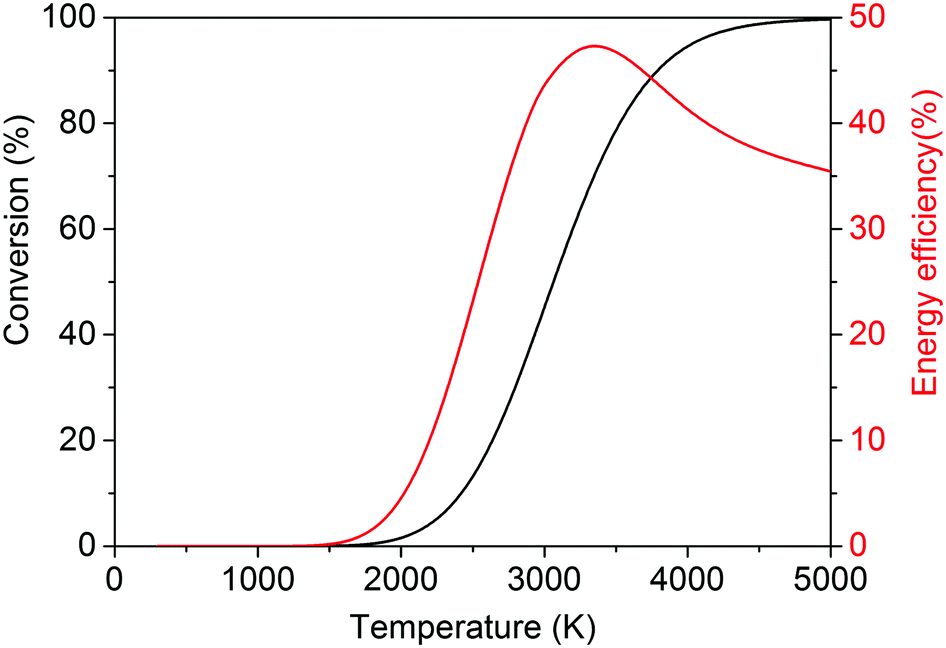
\includegraphics[width=0.7\linewidth]{chapter_3/figures/thermal_co2_conversion.png}
	\caption{Thermal conversion and energy efficiency of CO$_2$ splitting as a function of temperature. \cite{Snoeckx2017}}
	\label{fig:thermal_co2_conversion}
\end{figure}

It is no surprise why CO$_2$ splitting is greatly benefited by the use of catalysts, though this also increase the costs and complexity. The former is self explanatory, but the reason for increased complexity is that oxygen tends to remain on the catalyst surface, thus reducing its activity over time and therefore requiring regeneration \cite{Shin2017}. 

As a result, it is oftentimes more practical to include the use of a co-reactant to undergo the decomposition process. Ideally, this is done using a co-reactant with a higher Gibbs free energy ($\Delta G^\circ$), i.e. a less negative value \cite{jiang_xiao_kuznetsov_edwards_2010}.The equation for the $\Delta G^\circ$ is shown in equation \ref{eq:gibbs_free_energy_equation}. 

\begin{equation}
    \Delta G^\circ_f = \Delta H^\circ_f - T \Delta S^\circ
    \label{eq:gibbs_free_energy_equation}
\end{equation}

where $T$ is the temperature and  $\Delta S^\circ$ is the standard entropy of the system.

In simple terms, the $\Delta H^\circ_f$ denotes the relative stabilities of the compounds of the reaction while the $\Delta G^\circ$ describes if a given reaction will occur under a specified set of conditions. A negative $\Delta G^\circ$ means that the reaction is spontaneous. Figure \ref{fig:co2_stability} highlights a comparison between the $\Delta G^\circ$ of CO$_2$ and other common feedstock used. 

\begin{figure}[h!]
	\centering
	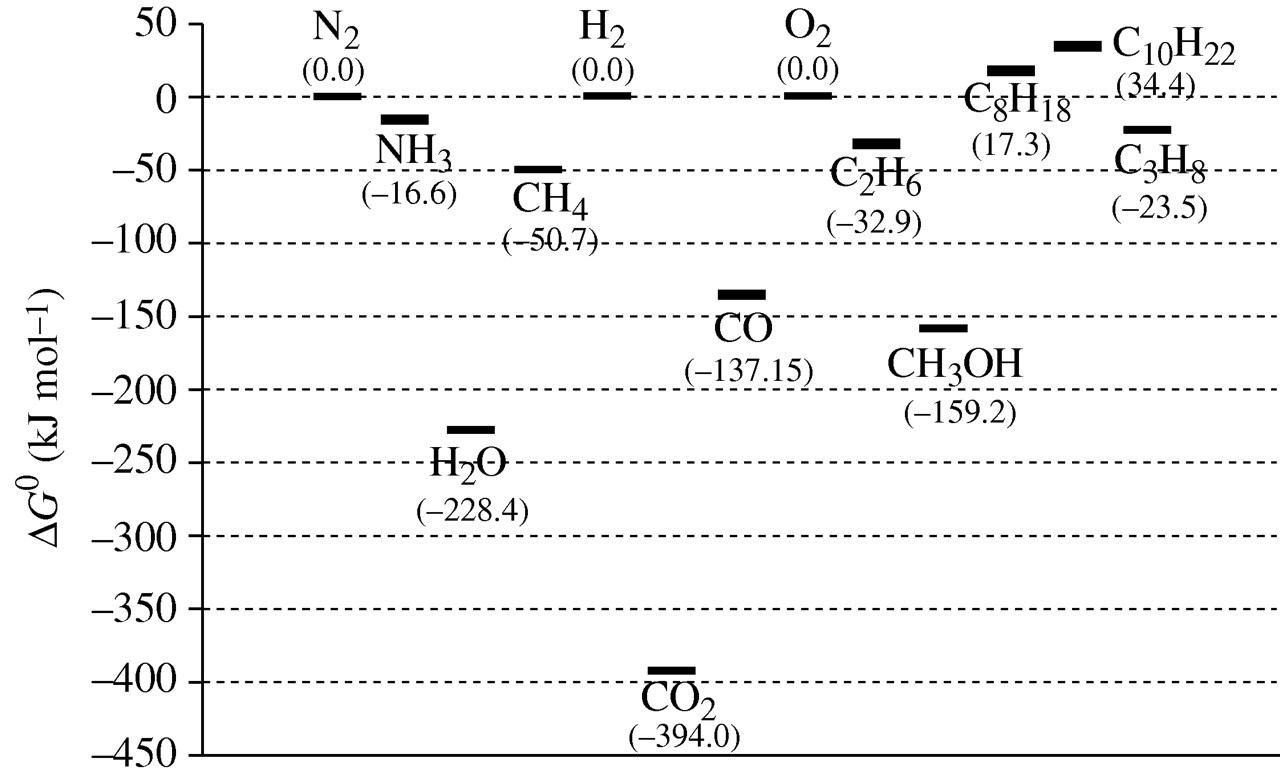
\includegraphics[width=0.83\linewidth]{chapter_3/figures/co2_stability.jpg}
	\caption{Gibbs free energy of formation for different chemicals based on data from the NIST database. \cite{jiang_xiao_kuznetsov_edwards_2010}}
	\label{fig:co2_stability}
\end{figure} 

In the literature, the most common co-reactants for CO$_2$ splitting are CH$_4$ and hydrogen gas (H$_2$). A brief overview of both these co-reactant processes are detailed below.

CH$_4$ is fairly abundant, and one common use of it is for the process of steam methane reforming (shown in equation \ref{eq:drm}) to produce syngas, which is a mixture of CO and H$_2$. Syngas is typically an intermediary for the production of ammonia, although it can also used to produce liquid hydrocarbons via the Fischer–Tropsch process. Hence, it is no surprise why there has been research into investigating CO$_2$ reformation of CH$_4$. This process is known as the dry reforming of methane, which is an endothermic reaction requiring $\Delta H^\circ_r  = 247.3$ kJ mol$^{-1}$ (approximately 2.5 eV molecule$^{-1}$). 

\begin{equation}
    \ce{CH_4 + CO_2 -> 2CO + 2H_2}
    \label{eq:drm}
\end{equation}

To push the equilibrium to the right, high temperatures (between 1000-1300 K) are required and typically this is done in the presence of a catalysts \cite{pakhare_spivey_2014}. Many different catalyst have been looked at, including the use of noble metals such as Rhodium (Rh) and Ruthenium (Ru), which have shown high activity and stability \cite{Rezaei2006, Rostrup-Nielsen1993}. However due to this costs, research into cheaper alternatives has been conducted. As an example  nickel (Ni) based catalysts have been shown to have a similar activity to that of the noble metals \cite{Ma2009}. Regardless of the catalyst used, the big limitation with this process is the formation of soot on the catalyst, which reduces yields and requires frequent regeneration cycles.

Besides the production of syngas, there are other uses for CH$_4$. The most common use of CH$_4$ by far is as a fuel source as it is the major constituent of natural gas. While not being particularly green in the long term, one viable use in the intermediary is to take excess electricity generated from renewable sources and green hydrogen to convert CO$_2$ into synthetic CH$_4$ (equation \ref{eq:sabatier_reaction}). This is an example of the Sabatier reaction, and has been in operation at a power-to-gas plant in Germany for nearly a decade \cite{etogas}.

\begin{equation}
    \ce{CO_2 + 4H_2 -> CH_4 + 2H_2O}
    \label{eq:sabatier_reaction}
\end{equation}

The benefit of this reaction is that it is exothermic, with a $\Delta H^\circ_r = -165.3$ kJ mol$^{-1}$ (approximately 1.7 eV molecule$^{-1}$), though achieving high conversion yields necessitates the use of a catalyst. Despite this benefit, the process presents two significant challenges.

The first issue arises from the fact that the majority of the global hydrogen supply is derived from steam methane reforming, a process that itself relies on CH$_4$ as a feedstock. The other issue to this process pertains to the efficiency of hydrogen utilisation; where unless water is the intended end product, approximately one-third of the hydrogen used contributes to the formation of a waste byproduct. This inefficiency becomes a major drawback when considering the scalability of the process for industrial applications.

A notable example where water is a desired end product is aboard the International Space Station. To ensure a sustainable water supply for astronauts, NASA employs a version of the Sabatier reaction represented in equation \ref{eq:sabatier_reaction_nasa} \cite{the_sabatier_system}.

\begin{equation}
    \ce{2H_2O ->[ electrolysis ] O_2 + 2H_2 ->[ respiration ] CO_2 + 2H_2 + 2H_2 (added) -> 2H_2O + CH_4 }
    \label{eq:sabatier_reaction_nasa}
\end{equation}

The process begins with the electrolysis of water, which generates breathable oxygen for the station’s crew. The resulting excess hydrogen gas is then combined with carbon dioxide, a byproduct of astronaut respiration, to produce water. This reaction also yields methane as a byproduct, which is subsequently vented into space.

Despite the effectiveness of this system in recycling resources, it remains partially dependent on external supplies; in particular, half of the hydrogen required is obtained through periodic resupply missions from Earth. Nevertheless, this represents a specialised use case that is not broadly applicable to the general CO$_2$ splitting process.



%This though is a simplification of the process, as it is most likely a two part mechanism \cite{rayne_2008}. The first half of the process would involve splitting the CO$_2$ into carbon monoxide (CO) and atomic oxygen (O) as seen in \ref{eq:co2_splitting}. The second step could take one of two possible pathways, however the most likely of the two would be the Boudouard reaction, seen in \ref{eq:boudouard_reaction}; however, this specific reaction is beyond the scope of this report.
%
%\begin{equation}
%    \ce{2CO_2 -> 2CO + O_2}
%    \label{eq:co2_splitting}
%\end{equation}
%\begin{equation}
%    \ce{2CO -> C + CO_2}
%    \label{eq:boudouard_reaction}
%\end{equation}
%
%Traditional thermal CO$_2$ splitting has not had much success to date, primarily due to the fact that CO$_2$ is an incredibly stable molecule with a Gibbs free energy of formation ($\Delta G^\circ$) of -394 kJ mol$^{-1}$. 
%
%The enthalpy of formation ($\Delta H^\circ_f$) of the reaction in \ref{eq:co2_splitting} is +283 kJ mol$^{-1}$, meaning that it is endothermic. Thus in order to make this reaction favourable, high temperatures are required. Figure \ref{fig:thermal_co2_conversion} highlights the conversion of such a reaction based on temperature, along with its corresponding energy efficiency \cite{Snoeckx2017}. This process could be improved by the presence of an active catalysts but this also increase the complexity and costs. 
%%Alternatively, one could remove the reactants
%
%\begin{figure}[h!]
%	\centering
%	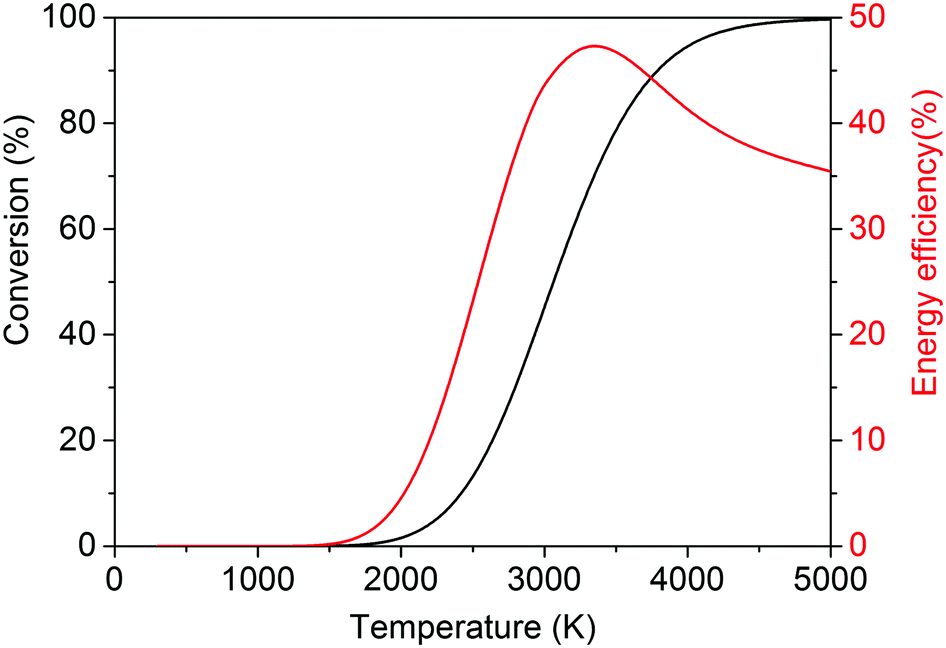
\includegraphics[width=0.6\linewidth]{chapter_3/figures/thermal_co2_conversion.png}
%	\caption{Thermal conversion and energy efficiency of CO$_2$ splitting as a function of temperature. \cite{Snoeckx2017}}
%	\label{fig:thermal_co2_conversion}
%\end{figure}
%
%Because of the low energy efficiency of pure CO$_2$ splitting, it is oftentimes more practical to include the use of a co-reactant. Ideally, this is done using a co-reactant with a higher Gibbs free energy (i.e. a less negative value) \cite{jiang_xiao_kuznetsov_edwards_2010}. In the literature, the most common co-reactants for CO$_2$ splitting are methane (CH$_4$, $\Delta G^\circ$ = -50.7 kJ mol$^{-1}$) and hydrogen (H$_2$, $\Delta G^\circ$ = 0.0 kJ mol$^{-1}$).




%
%
%As for using H$_2$ as a co-reactant to CO$_2$ splitting, this process is known as the Sabatier reaction. The reaction, seen in \ref{eq:sabatier_reaction}, is typically to generate synthetic natural gas but has other uses such as the production of water on the international space station \cite{the_sabatier_system}.
%
%\begin{equation}
%    \ce{CO_2 + 4H_2 -> CH_4 + 2H_2O}
%    \label{eq:sabatier_reaction}
%\end{equation}
%
%The reaction is exothermic, with a $\Delta H^\circ_f$ = -165.3 kJ mol$^{-1}$, but does require a catalyst in order to achieve high conversion yields. Nonetheless, there are two issues with this process. The first being, unless water is the desired end product, a third of the H$_2$ used goes towards the creation of a waste product; not ideal when using this process at scale. The other issues has to do with the fact that most of the world's supply of H$_2$ comes from the process of steam reforming, which produces CO$_2$ as a by-product. 

\section{Plasma Driven Process}

As highlighted above, there are several shortfalls with the conventional process of CO$_2$ splitting. This is where the use of plasma-assisted CO$_2$ decomposition, specifically using non-thermal plasmas (i.e. generated by electric means), can be beneficial. In these plasmas, the electrons attain significantly higher temperatures compared to the ions or the background gas. These energetic electrons 
can effectively dissociate molecules, including highly stable compounds such as CO$_2$
 in the plasma can dissociate molecules, even highly stable ones such as CO$_2$, under standard temperature and pressure conditions \cite{Snoeckx2017}. 

Because of this behaviour, there is no need for heat or pressurised reactors, thereby reducing both complexity and associated costs. Another advantage of this method is its ``turn-key" operation, as the plasma can be instantaneously switched on and off with minimal stabilisation times. There is also no need for rare earth metals to be used as catalysts, and it has been shown that plasma reactors can have good scalability as shown by Kogelschatz in \cite{kogelschatz_2003}. 

In the plasma-assisted decomposition process, multiple reaction pathways are available for CO$_2$ splitting which are discussed below. It is important to note that, throughout this discussion, all energy values will be expressed in the units eV per molecule (simply written as eV), rather than kJ mol$^{-1}$, as it is the common nomenclature in the plasma literature. or reference, the CO$_2$ splitting reaction shown in equation \ref{eq:co2_splitting} requires about 2.93 eV.

\begin{figure}[h!]
	\centering
	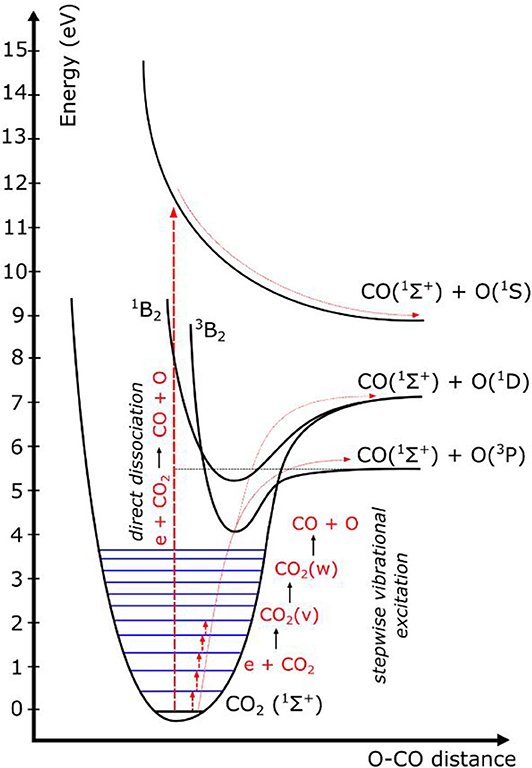
\includegraphics[width=0.6\linewidth]{chapter_3/figures/co2_dissociation_energies.jpg}
	\caption{Schematic of the electronic and vibrational levels for CO$_2$\cite{Bogaerts2020}.}
	\label{fig:co2_dissociation_energies}
\end{figure}

One of the pathways for dissociation is via direct electron impact (shown dashed red line in figure \ref{fig:co2_dissociation_energies}), whereby an electron with sufficient energy collides with the CO$_2$ molecules to break the bond directly (equation \ref{ce:direct_electron_dissociation}) \cite{Bogaerts2020}. This pathway requires electron energies of more than 7 eV  to occur. However, it is also possible to break the \ce{C=O} bond using stepwise vibrational excitation (equation \ref{ce:step_wise_electron_dissociation}) \cite{Bogaerts2020}. This occurs when the CO$_2$ molecules absorbs a series of energy quanta, either through collisions or via photons, to transition into higher vibrational state and eventually lead to the bond breaking. This stepwise approach requires minimum energy levels of at 5.5 eV, which provides a more efficient path for the dissociation.

\begin{equation}
    \ce{CO_2 + e^{-} -> CO + O + e^{-}}
    \label{ce:direct_electron_dissociation}
\end{equation}

\begin{equation}
\begin{aligned} 
    \ce{CO_2 + e^{-} & -> CO_2^*(v) \\ CO_2^*(v) + e^{-} & -> CO_2^*(w) \\ CO_2^*(w) + e^{-} & -> CO + O + e^{-}}
    \label{ce:step_wise_electron_dissociation}
\end{aligned} 
\end{equation}

While the two aforementioned approaches tend to be the dominant pathways, it is also possible for vibrationally excited CO$_2$ molecules to undergo dissociation via collisions with excited molecules, with energies typically $<$ 1 eV (equation \ref{ce:vibrational_exitation_oxygen}) \cite{Chen18} . 

\begin{equation}
    \ce{CO^*_2 + O -> CO + O_2}
    \label{ce:vibrational_exitation_oxygen}
\end{equation}


Once the splitting CO$_2$ molecule occurs, it is often accompanied by the recombination of the oxygen atoms (equation \ref{ce:oxygen_recombination}) \cite{Chen18}. Note that M is a particle from the background gas.

\begin{equation}
    \ce{M + O + O -> O_2 + M}
    \label{ce:oxygen_recombination}
\end{equation}

%The dominant pathway is via electron-impact dissociation, with an energy threshold around 5.5 eV per molecule; which corresponds to the energy required to break the \ce{C=O} bond \cite{Bogaerts2020};. This is often accompanied by the recombination of the oxygen atoms \cite{Chen18}. This is shown in equations \ref{ce:electron_dissociation} and \ref{ce:oxygen_recombination} respectively.
%
%\begin{equation}
%    \ce{CO_2 + e^{-} -> CO + O + e^{-}}
%    \label{ce:electron_dissociation}
%\end{equation}
%
%
%
%
%Though, it is also possible splitting to occur by stepwise vibrational excitation of the CO$_2$ molecules as they collide with low energy electrons and excited molecules (typically less than 1 eV) \cite{Chen18}. These are also shown in equations \ref{ce:vibrational_exitation_oxygen} and \ref{ce:vibrational_exitation_electron} respectively.
%
%
%
%\begin{equation}
%    \ce{CO^*_2 + e^{-} -> CO + O + e^{-}}
%    \label{ce:vibrational_exitation_electron}
%\end{equation}

There are several different methods to generate plasma for CO$_2$ splitting in the literature, however the most common are: dielectric barrier discharges (DBD), gilding arc discharges (GA), and radio frequency (RF)/microwave (MW) discharges. As mentioned in the previous chapter, arc discharges are excluded from the scope of this research due to concerns related to electrode sputtering. Therefore, the subsequent discussion in this section will focus exclusively on DBD, RF, and MW discharges.

These processes are typically characterized and evaluated using two primary metrics: \textit{conversion efficiency} and \textit{energy efficiency}. The conversion efficiency ($\rchi_{CO_2}$) denotes the fraction of CO$_2$ used by the splitting process, and can be defined as:

\begin{equation}
    \rchi_{CO_2} = \frac{n_{start} - n_{end}}{n_{start}}
\end{equation}

where $n$ is the number of moles of CO$_2$. While it is tempting to think of the conversion efficiency as equivalent to the yield, it is not. This is because the yield only measures the fraction of the desired product produced, whereas the conversion efficiency could include unwanted byproducts which have consumed the CO$_2$.

On the other hand, i ($\eta_{CO_2}$) corresponds to the fraction of input energy that went into splitting the CO$_2$ molecules. This can be expressed as:

\begin{equation}
    \eta_{CO_2} = \frac{\rchi_{CO_2} \Delta H^{\circ}_r}{SEI}
\end{equation}

where $\Delta H^{\circ}_r$ corresponds to the enthalpy change for CO$_2$ dissociation (which is 2.93 eV molecule$^{-1}$) and $SEI$ is the specific energy input. 

The $SEI$ describes the energy supplied per unit of CO$_2$ processed in plasma conversion \cite{Hegemann2023}. It can be calculated as the ration between the discharge power and the gas flow rate. While discharge power is almost always measured in watts (W), there are many different standard units for measuring flow rates of gases. For this report, all flow rates are measured in standard cubic centimetres per minute (sccm). Occasionallu, standard litres per minute (slm) is used which is equivalent to 1000 sccm.

With discharge power (P) and flow rate (Q), the SEI (in eV molecule$^{-1}$) can be calculated as follows \cite{Ozkan2015}:

\begin{equation}
    SEI = \frac{P \text{ (Js$^{-1}$)}}{Q \text{ (cm$^{3}$ min$^{-1}$)}} \times \frac{60 \text{ (s min$^{-1}$)} \times 6.24 \times 10^{18} \text{(eV J$^{-1}$)} \times 24000 \text{ (cm$^{3}$ mol$^{-1}$)}}{6.022 \times 10^{23} \text{ (molecule mol$^{-1}$)}} 
    \label{eq:sei_expanded}
\end{equation}

Note that the value 24000 cm$^{3}$mol$^{-1}$ is derived from the ideal gas law at atmospheric pressure and at 293K. 

Equation \ref{eq:sei_expanded} simplifies to:

\begin{equation}
    SEI = \frac{P}{Q} \times 14.926 \text{ (eV molecule$^{-1}$)}
    \label{eq:sei}
\end{equation}

Snoeckx and Bogaerts compiled a list of various plasma reactors for CO$_2$ conversion, and evaluated their conversion and energy efficiencies \cite{Snoeckx2017}. An illustration of the result can be seen in figure \ref{fig:conversion_and_energy_efficiencies}. 

\begin{figure}[h!]
	\centering
	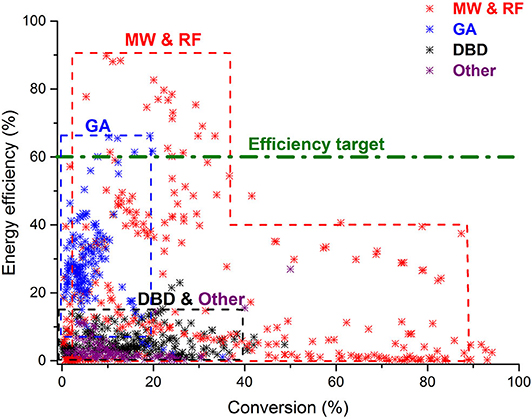
\includegraphics[width=0.7\linewidth]{chapter_3/figures/conversion_and_energy_efficiencies.jpg}
	\caption{Comparison of conversion and energy efficiencies for various CO$_2$ splitting plasma reactors \cite{Snoeckx2017}.}
	\label{fig:conversion_and_energy_efficiencies}
\end{figure}

From the figure \ref{fig:conversion_and_energy_efficiencies}, it is evident that one of the most extensively studied processes for CO$_2$ splitting involved DBD reactors. This is not surprising given that DBD reactors have already had industrial success in areas related to ozone production and volatile organic compound (VOC) removal \cite{Kogelschatz2003}. Nonetheless, they seem to have relatively poor performance, which makes it hard to justify them for industrial applications. GA plasmas perform better than DBD reactors when it comes to energy efficiency. However, they struggle to get a conversion efficiency greater 20\%, most likely due to the fact that the amount of gas passing through the the arc of plasma is minimal.

RF and MW plasmas by contrast appear to have a wide spectrum of results. From reactors that trade off low conversion for high energy efficiencies and vice versa, to designs that are located in the middle of both parameters. A lot of these RF and MW plasma reviewed operated at sub-atmospheric pressure. Because of the promise shown by MW reactors, the rest of this chapter will highlight examples from the literature.

A key point to highlight from Figure \ref{fig:conversion_and_energy_efficiencies} is the proposed energy efficiency target of 60-80\%. Snoeckx and Bogaerts argue that this efficiency range should serve as the benchmark for plasma-assisted conversion to be considered a competitive and viable alternative to conventional methods. The rationale behind this target is to align with the efficiency of electrochemical water splitting, which typically achieves energy efficiencies of approximately 65-75\%, and solar-to-fuel conversion technologies, which reach efficiencies of around 20\%. Assuming the reactors are powered by solar panels with a 25\% efficiency, this results in an overall solar-to-fuel efficiency of approximately 15-20\%.

Many MW plasma experiments utilise a structure as seen in figure \ref{fig:mw_reactor}, called surface-wave discharges. Gas is typically fed through a tube (typically quartz), coupled with an external wave guide where the microwave discharge is generated. The typical frequencies in such experiments are 915 MHz or 2.45 GHz, which are approved for industrial applications, and which influence the dimensions of the setup. 

\begin{figure}[h!]
	\centering
	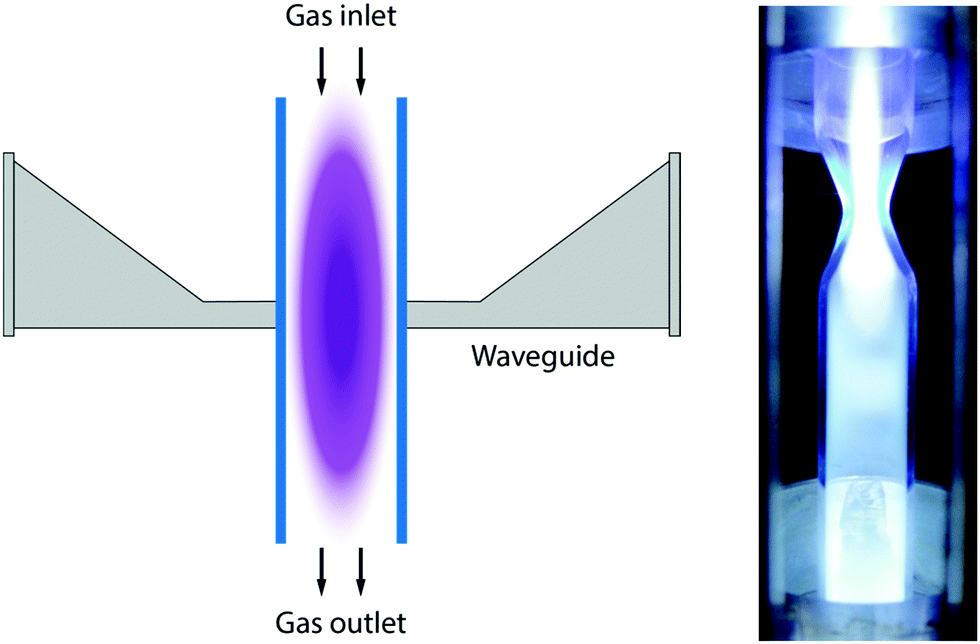
\includegraphics[width=0.8\linewidth]{chapter_3/figures/mw_reactor.png}
	\caption{Schematic of microwave reactors for CO$_2$ splitting \cite{Snoeckx2017}.}
	\label{fig:mw_reactor}
\end{figure}

Bongers et al used one such a reactor \cite{Bongers2015DevelopmentsIC} at a frequency of 915 MHz at approximately 150 Torr. They were able to obtain a conversion efficiency of up to 23\% at an energy efficiency of 36\%, although  energy efficiency of 50\% could be achieved at lower powers and reduced conversion. A complexity of their setup was that it required a specialised configuration where the gas was supersonically expanded in the plasma.

A more typical configuration was used by Silva et al \cite{Silva2014}, the experiment was operated at 2.45 GHz with a pulsed microwave generator operating at low pressure (1-10 Torr). They used a gas mixture of CO$_2$ with 5\% nitrogen (N$_2$), and were able to get conversion efficiency of 80\% with a steady energy efficiency of around 12\%. 

As with thermally driven processes, plasma-assisted CO$_2$ splitting commonly incorporates co-reactants. While inert gases such as argon (Ar) and helium (He) are typically used, nitrogen (N$_2$) is also frequently employed due to its widespread availability and cost-effectiveness. A significant drawback of using N$_2$ is its higher conversion rate compared to CO$_2$, which promotes the formation of undesirable byproducts such as NO$_2$, NO, and N$_2$O \cite{Qin2018}.  

Due to their chemical inertness, noble gases do not contribute to the formation of unwanted byproducts. In plasma systems, their primary role is to act as an electron source. The use of inert gases is particularly advantageous because they lack vibrational and rotational energy levels, minimising energy loss through quenching and thereby facilitating plasma sustainment.

Additionally, studies have demonstrated that the breakdown voltage is reduced when CO$_2$-Ar or CO$_2$-He mixtures are utilised \cite{Ramakers2015}, while the increased electron density enhances the frequency of collisions \cite{Qin2018, Ramakers2015}. When selecting between these two inert gases, argon (Ar) is the more cost-effective option. However, helium (He) possesses a higher ionisation potential (24.6 eV) than argon (15.8 eV), which accounts for the higher electron temperature observed in He plasmas \cite{Qin2018, Jeroen_Jonkers_2003}.

Other gases have been used as co-reactants, including H$_2$ by Chen et al \cite{chen2017role}. They used a surface waveguide with a frequency of 915 MHz, at a pressure of around 30 Torr. The H$_2$ was initially produced through the decomposition of water, after which the Sabatier reaction took place (equation \ref{eq:sabatier_reaction}). Using a NiO/TiO catalyst, the researchers achieved a CO$_2$ conversion efficiency of 22\% and an energy efficiency of 52\%.

Additionally, CH$_4$ has been explored as a co-reactant by Chun et al \cite{Chun2017}. Their study employed a plasma torch operating at 2.45 GHz, featuring a structure similar to the surface waveguides depicted in figure \ref{fig:mw_reactor}, with modifications in the form of channels within the quartz tube to induce gas swirling. With this, they were able to get conversion efficiencies of 68.4\% for CO$_2$ and 96.8\% for CH$_4$. While no direct energy efficiency value was provided, rough calculations based on the reported parameters suggest an efficiency of approximately 33\%. A big advantage of this process had to do with the fact that it is one of the few processes that operates at atmospheric pressure (760 Torr).

All the previously discussed examples have involved gaseous reactants. However, it is also possible for the co-reactants in the CO$_2$ decomposition process to be liquids. Research in this area has historically been limited due to the fact that these liquid co-reactants are typically organic compounds, making them unsuitable for low-pressure operations (as seen in many of the previous examples) due to vapor pressure constraints \cite{Bruggeman2016}. Nevertheless, with the advances in plasma reactors operating at atmospheric pressure, these plasma–liquid systems have become an interesting area of research. A key advantage is that this leads to a broader range of possible reactions with CO$_2$, allowing for the production of a wider array of desired end products. Additionally, if the end product is also a liquid, it allows for easier separation of the product from the waste reactants. 

\begin{figure}[h!]
	\centering
	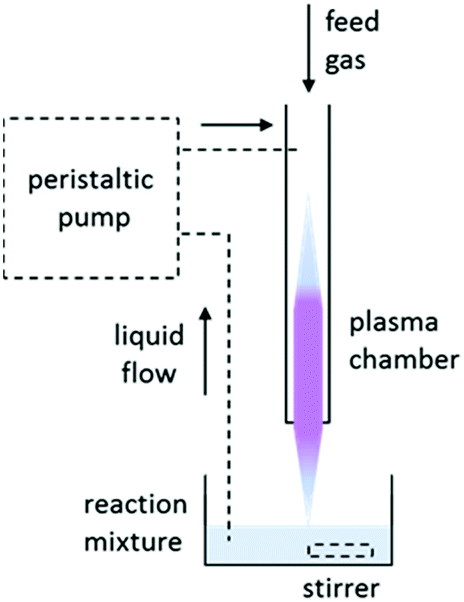
\includegraphics[width=0.35\linewidth]{chapter_3/figures/rf_torch_with_liquid.png}
	\caption{Illustration of the experimental setup by Gorbanev et al \cite{Gorbanev2017}.}
	\label{fig:rf_torch_with_liquid}
\end{figure}


One example of research into plasma–liquid systems was done by Gorbanev et al \cite{Gorbanev2017}. They tested three different organic solutions (dehalogenation of iodoarenes, 5-exo-trig cyclisation, and trifluoromethylation with the Togni-II reagent) using a DBD reactor operating at a frequency of 25 kHz. An illustration of the apparatus used is shown in figure \ref{fig:rf_torch_with_liquid}.  The feed gas included a CO$_2$-He mixture, with yields reaching up to 95\% after 30 mins. However, there were a lot of variations in the results, and even the authors noted that the results were only preliminary with more work required to optimise reaction efficiency.

\begin{figure}[h!]
	\centering
	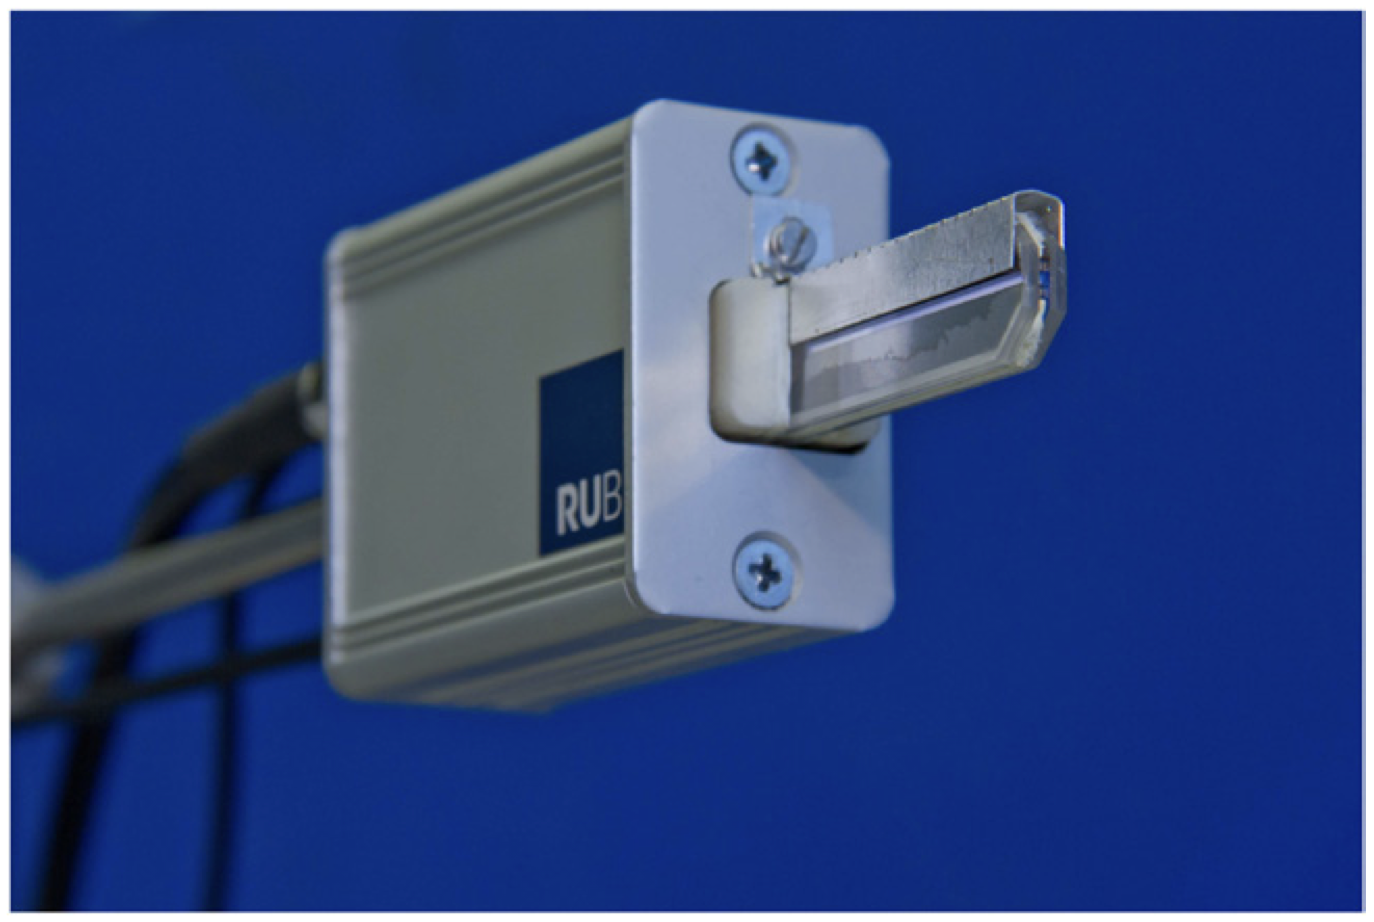
\includegraphics[width=0.75\linewidth]{chapter_3/figures/COST_jet.png}
	\caption{Photograph of COST jet \cite{Golda2016}.}
	\label{fig:COST_jet}
\end{figure}

A more recent development was reported by  Xu et al \cite{Xu2021}, utilising the COST microplasma jet developed as part of a European COST (Cooperation in Science and Technology) initiative \cite{VonDerGathen2008}. The reactor was a capacitively coupled design that operates at 13.56 MHz, seen in figure \ref{fig:COST_jet}. The schematic of experimental setup by Xu et al is shown in figure \ref{fig:han_epoxidation_setup}. The benefit of the COST jet is its ability to operate at atmospheric pressure, making it suitable for chemical synthesis applications.

Their experimental setup incorporated a CO$_2$-He mixture  with a liquid co-reactant, \textit{trans}-stilbene. The reaction yielded an epoxide (which are a popular compound used for detergents, adhesives, and plastics) and the waste gas CO. This reaction can be seen below, and the chemical structure of the compounds are shown in figure \ref{fig:epoxidation_diagram}.

\begin{equation}
    \ce{CO$_2$  (g) + C_6H_5CH=CHC_6H_5 (l) ->[plasma] CO (g) + C_6H_5CH=CHC_6H_5O (l)}
\end{equation} 

\begin{figure}[h!]
    \centering
    \begin{subfigure}[b]{0.35\textwidth}
        \centering
        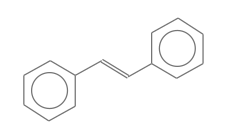
\includegraphics[width=\textwidth]{chapter_3/figures/ts.png}
        \caption{}
    \end{subfigure}
    \quad\quad
    \begin{subfigure}[b]{0.35\textwidth}  
        \centering 
        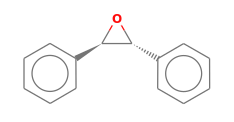
\includegraphics[width=\textwidth]{chapter_3/figures/tse.png}
        \caption{}
    \end{subfigure}

    \caption{\small Chemical structure of \textit{trans}-stilbene (a) and \textit{trans}-stilbene oxide/epoxide (b).} 
    \label{fig:epoxidation_diagram}
\end{figure}

%\begin{figure}[h!]
%	\centering
%	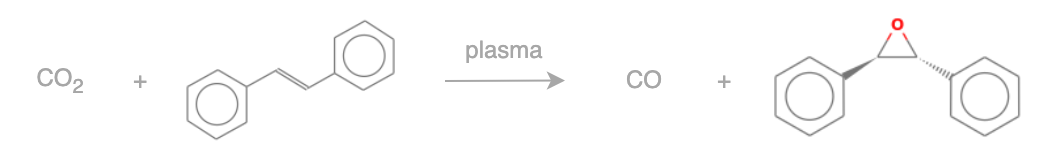
\includegraphics[width=0.9\linewidth]{chapter_3/figures/epoxidation_diagram.png}
%	\caption{Chemical structure of \textit{trans}-stilbene and \textit{trans}-stilbene oxide (epoxide).}
%	\label{fig:epoxidation_diagram}
%\end{figure}


In the experimental setup, the plasma jet was positioned 4 mm above the surface of the liquid. The researchers achieved a consistent epoxide yield of approximately 75\%, with a slightly lower conversion efficiency of around 70\%. However, the study did not report energy efficiency values, as the specific power input of the reactor was not disclosed.

This approach appears to be promising, particularly since it operates at atmospheric pressure. However, one limitation of the process is temperature plays an important role in the efficiency of the reaction. The optimal reaction efficiency was observed at approximately -25 $^\circ$C, though it remains viable at room temperature, with only a 5\% reduction in yield.

\begin{figure}[h!]
	\centering
	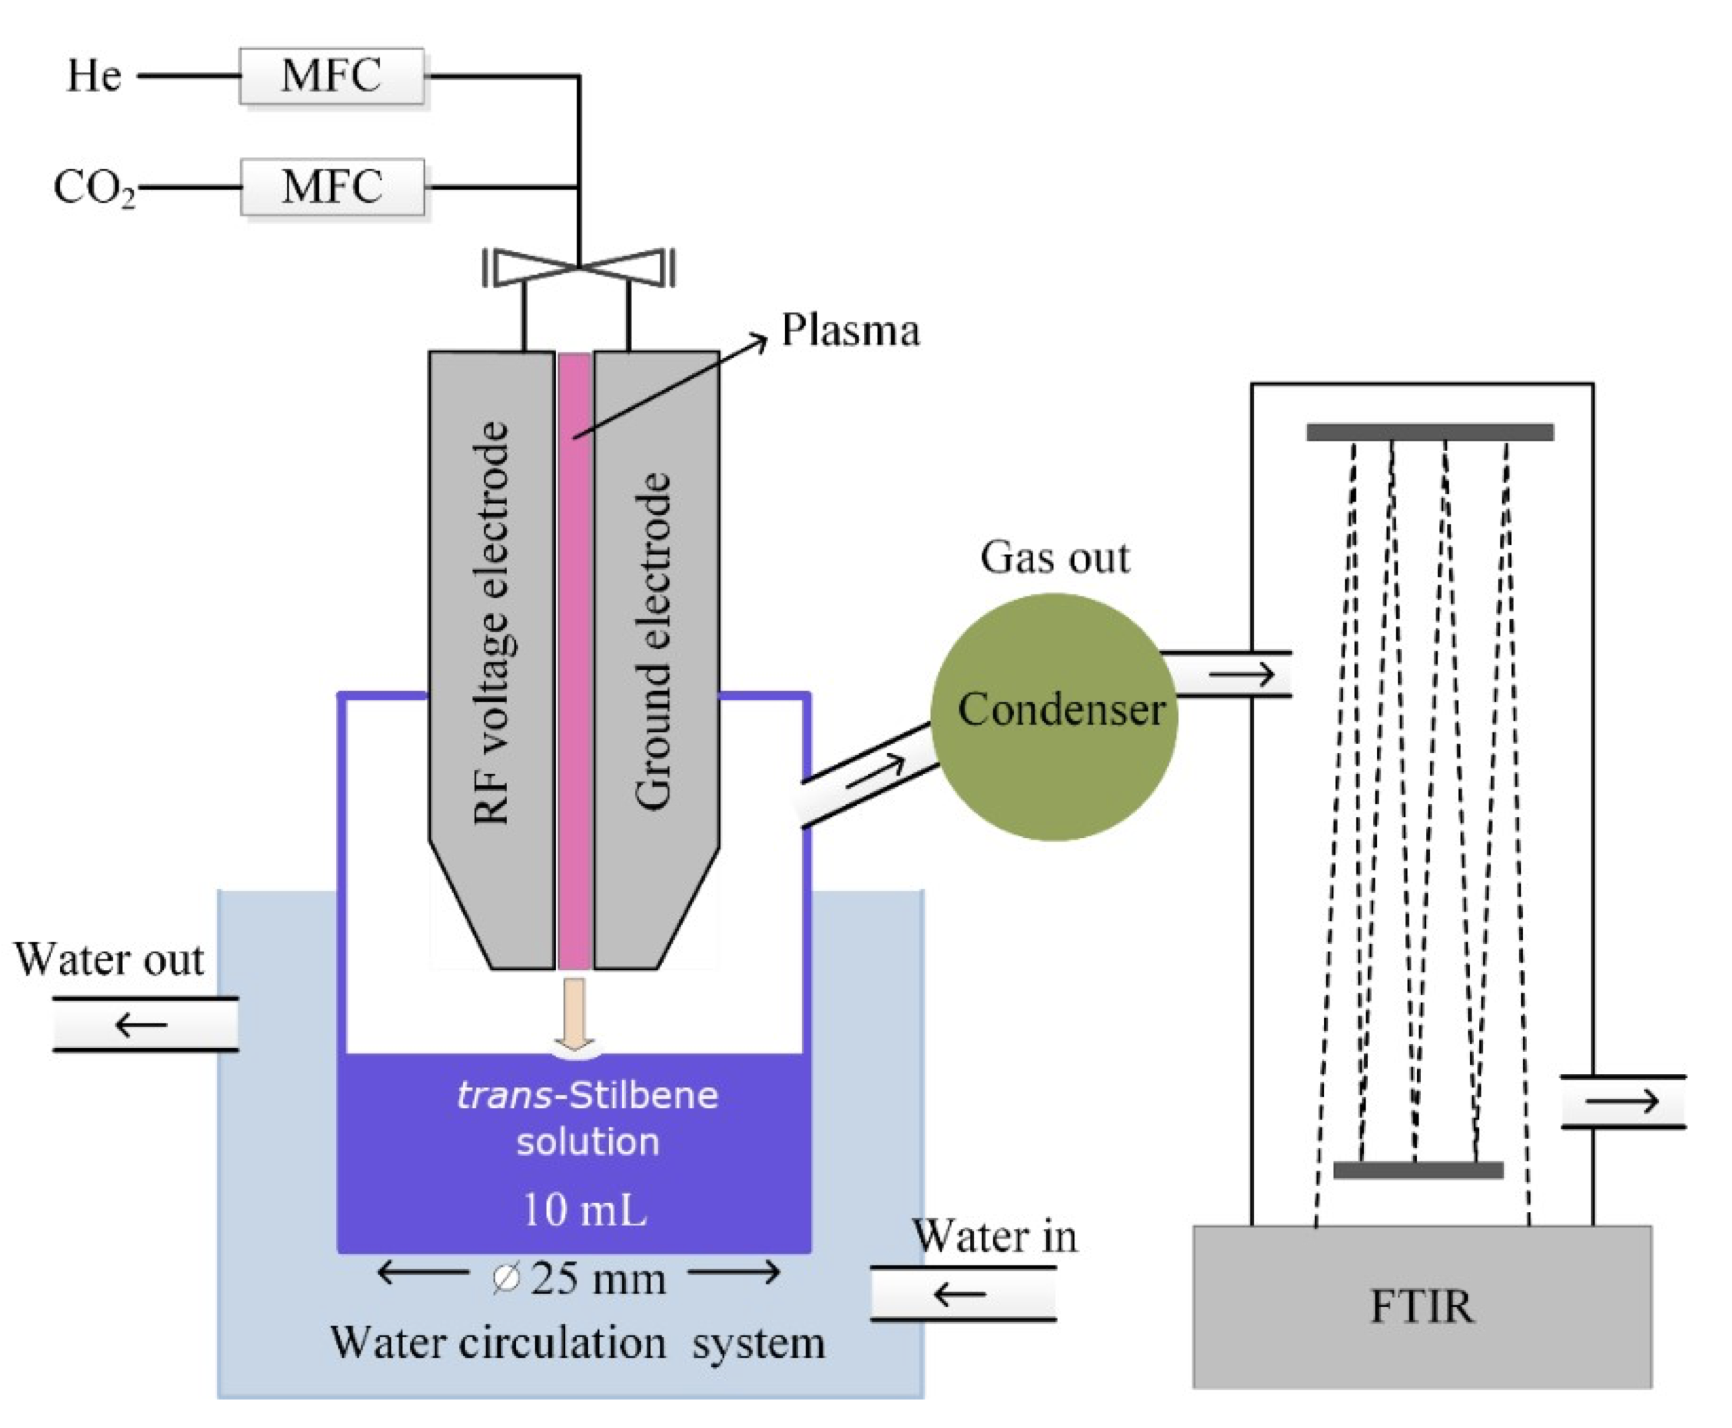
\includegraphics[width=0.75\linewidth]{chapter_3/figures/han_epoxidation_setup.png}
	\caption{Schematic of experimental setup by Xu et al \cite{Xu2021}.}
	\label{fig:han_epoxidation_setup}
\end{figure}

This report aims to build on this process while addressing key limitations identified by Xu et al. One of the primary concerns is the use of helium as the feed gas, which is vented into the atmosphere. Given that helium is an expensive noble gas, it would be beneficial to develop a system that allows for its reuse within the plasma reactor. Alternatively, the feasibility of substituting helium with a more cost-effective gas, such as argon could be investigated. The reaction also produces CO as a byproduct, which is a valuable industrial gas in itself, hence its extraction for secondary reactions could be another area of interest.

The other challenge encountered by Xu et al related to the distance of the plasma nozzle to the surface of the treated liquid. To achieve the ideal reaction efficiency, this distance should be minimised. However, reducing the nozzle-to-liquid gap led led to an increased rate of solvent evaporation, making it difficult to maintain a constant distance throughout the process. This  motivated the exploration of an alternative reactor design that allows the liquid to remain in closer proximity to the plasma. The details of this plasma device are discussed in the following chapter.




%Nonetheless, other designs for RF/microwave discharges exist such as the one developed by Xu et al \cite{Xu2021}. Their design utilised a co-reactant called \textit{trans}-stilbene. Unlike the co-reactants previously mentioned, which were  gaseous, \textit{trans}-stilbene is a liquid. Because of this, the plasma had to directly contact the solution, which was achieved via a plasma jet reactor. The jet nozzle had to be place 4 mm above the surface of the liquid, and the final product of this reaction was CO and epoxides (a popular compound use for detergents, adhesives, and plastics). The authors were able to obtain a 75\% yield on epoxides and a splitting of approximately 70\% of the CO$_2$ in the plasma. As such, this will be the process that is emulated in this report.


